\section{Introduction}
The function of rs-fMRI scans is to study neuronal activities across time by tracking changes
in the BOLD signal while the subject is in a task-negative state. Thus, raw functional images
are 4D where each dimension represents the height, width, depth/number of brain slices and
time of repetition of each subject/sample.\\

However, in this research, we will not use fMRI image data rather we will represent fMRI
scans as mean time-series data from particular ROIs. These specific ROIs are selected using a
functionally parcellated brain atlas. Each of these atlases use different approaches to segment
the entire brain into several ROIs. The various steps of our proposed methodology are
discussed in this chapter in detail.\\

\section{Overview of ASD Detection Framework}

Figure \ref{fig:3.1} represents the basic steps of the proposed autism detection framework. Preprocessed rs-fMRI data of the ABIDE dataset are obtained from the Preprocessed Connectome Project (\Gls{PCP}). The CPAC preprocessing pipeline is applied for nuisance signal removal and attaining quality criteria. After that, certain brain areas of interest are considered using brain atlases. These brain
atlases serve as a mask that extracts signals of certain predefined ROIs from the preprocessed
dataset. A connectivity matrix is created using tangent space embedding that provides
information about the intensity of correlation between each ROI pairs. Finally, the
connectivity matrix is collapsed to form a 1D vector removing redundant elements. This
feature vector is provided as input to the deep learning classifier. During training, the feature vector along with the corresponding label of each sample (i.e,
either autism or control) are provided as input to the DNN classifier. Using this trained
classifier, testing is executed where the labels of each test sample were determined by the
classifier.\\

\begin{figure}[h]
\centering
\includegraphics[width=\textwidth]{figures/Figure 3.1.png}
\caption{Steps of the proposed autism spectrum disorder (ASD) detection framework.}
\label{fig:3.1}
\end{figure}

\section{Detailed Explanation of the ASD Detection Framework}

The explanation of each steps conducted in the entire process of ASD detection is represented in the following subsections along with their implementation details.\\

\subsection{Preprocessing}
The preprocessed fMRI dataset of the ABIDE repository \cite{di2014autism, abide} was collected from the preprocessed connectome project (PCP) \cite{craddock2013neuro}. The configurable pipeline for the analysis of connectomes (CPAC) preprocessing pipeline was used, which included slice timing correction, motion correction, intensity normalization, nuisance signal removals, such as respiration, heartbeat, low-frequency scanner drifts, global mean signal regression, head motion, etc. The preprocessed data were band-pass filtered (0.01–0.1 Hz) and spatially registered to MNI152 template space. Table \ref{tab:3.1} contains an overview of the preprocessing steps included in
the CPAC pipeline.\\

\begin{table}[h!]
\begin{center}
    \caption{Steps of CPAC preprocessing pipeline.}
    \label{tab:3.1}
\begin{tabular}{|l|l|lll}
\cline{1-2}
\multicolumn{1}{|c|}{\textbf{Steps}} & \multicolumn{1}{c|}{\textbf{CPAC}} &  &  &  \\ \cline{1-2}
\multicolumn{2}{|c|}{\textbf{Regressor}}                                  &  &  &  \\ \cline{1-2}
Motion                               & 24-param                           &  &  &  \\ \cline{1-2}
Tissue signals                       & CompCor (5 PCs)                    &  &  &  \\ \cline{1-2}
Low-frequency drifts                 & Linear and quadratic trends        &  &  &  \\ \cline{1-2}
\multicolumn{2}{|c|}{\textbf{Registration from original to MNI152}}       &  &  &  \\ \cline{1-2}
Functional to Anatomical transform   & boundary-rigid body (BBR)          &  &  &  \\ \cline{1-2}
Anatomical to Standard transform     & ANTs                               &  &  &  \\ \cline{1-2}
\end{tabular}
\end{center}
\end{table}

Detailed information regarding algorithms, strategies, parameters used, and software implemented can be obtained from \cite{abidepreprocessed}.

\subsection{Time-series Extraction from ROIs using Brain Atlas}

The accuracy of ASD and control classification largely depends on the brain atlas used to
extract specific regions of interest (ROI) from whole-brain fMRI volumes. The hypothesis is
to use a parcellation atlas, either by data-driven method or from the predefined ones such
that, the selected ROIs contain regions comprising the most discriminative features between
an autistic brain and control brain. In this study, we consider four standard predefined brain
atlases among which three are functional (BASC, Power, CC200) and one is structural
(AAL). A pictorial representation of time-series extraction from fMRI volume using brain
atlas is visualized in Figure \ref{fig:3.2}.\\
\newpage
\begin{figure}[h]
\centering
\includegraphics[width = \textwidth]{figures/Figure 3.2.png}
\caption{Time-series Extraction from 4D fMRI Volume using Brain Parcellation Atlas.}
\label{fig:3.2}
\end{figure}

\subsubsection{Selection of Predefined Atlases}

\begin{itemize}
    \item \textbf{AAL – Automated Anatomical Labelling:} \\
    It is a structural atlas comprising 116 ROIs defined from the anatomy of a reference
object in \cite{tzourio2002automated}. The 116 regions are defined by AAL atlas along the three anatomical
planes (Axial, Sagittal and Coronal) as shown in Figure \ref{fig:3.3} for visualization purpose
where ROIs are represented in continuous colours.

\begin{figure}[h!]
\centering
\includegraphics[]{figures/Figure 3.3.png}
\caption{Automated Anatomical Labelling (AAL) atlas.}
\label{fig:3.3}
\end{figure}
\newpage
 \item \textbf{BASC – Bootstrap Analysis of Stable Clusters:} \\
This multiscale functional brain parcellation atlas was generated from rs-fMRI images
from about 200 young healthy subjects using a method called bootstrap analysis of
stable clusters in \cite{bellec2010multi}. It consists of a different number of ROIs {36, 64, 122, 197,
325, 444}. BASC atlas with 122 ROIs is utilized in this study. The visual
representation of this atlas is shown in Figure \ref{fig:3.4} using continuous colours to
represent ROIs.

\begin{figure}[h!]
\centering
\includegraphics[]{figures/Figure 3.4.png}
\caption{Bootstrap Analysis of Stable Clusters (BASC) atlas.}
\label{fig:3.4}
\end{figure}

\item \textbf{CC200—Craddock 200:} \\
The CC200 functional brain parcellation atlas was generated by normalized cut
spectral clustering of the entire brain into 200 spatially-constrained regions of
homogeneous functional activity by Craddock et al. in \cite{craddock2012whole}.

\item \textbf{Power:} \\
Power atlas comprising 264 ROIs were defined by local graph-connectivity by Power
et al. in \cite{power2011functional}.
\end{itemize}

All the brain images used in this section were generated by the Nilearn Python library using
the plotting function. Nilearn is a python module for easy and fast statistical learning on
neuroimaging data which provides tools and functions to enable versatile analyses of brain
volumes in \cite{nilearn}.

\subsubsection{Mean Timeseries Extraction of ROIs from 4D fMRI Brain Volume}
A single fMRI scan is a 4D time-series including three spatial dimensions and time. In order to extract
and transform meaningful features from such complicated multidimensional data in a
structured way and to store it in a convenient format, certain pre-defined regions of interests
(ROIs) are considered.\\

In other words, instead of working with the entire time series obtained from every brain
voxels directly, we consider certain brain regions comprising several voxels and extract mean
time-series signals from voxels enclosed within those regions. To accomplish this, we use a
brain atlas where the brain regions or the ROIs are already defined. Applying a brain atlas on
4D fMRI scans can be imagined as overlaying a series of 3D grids that act like a mask and
selects which cubes or voxels to sample from at every time point.\\

Thus, original 4D fMRI data of a single subject with dimensions (H, W, D, T) gets
transformed to 2D data with dimensions (T, N) where H, W, D, T represents height, width,
depth or number of slices, time points of the image volume and number of ROIs, respectively. Now, this 2D data can form a TxN matrix where each row represents time points and each
column represent features derived from rs-fMRI data.\\

However, the whole process of extracting mean time-series signals applying brain atlas on preprocessed rs-fMRI data requires a huge amount of memory space. Due to hardware and memory constraints, we utilized pre-extracted time-series data. In this study, mean time-series signals containing CC200 and AAL defined ROIs were obtained directly from PCP \cite{abidepreprocessed}, and those containing BASC and Power atlas defined ROIs were collected from \cite{dadi2019benchmarking}. Thus, the (T, N) dimension in our study was (196, 200), (196, 116), (196, 122), and (196, 264) for CC200, AAL, BASC, and Power, respectively, since scans were generated for 196 time points in each case.

\subsection{Building Functional Connectivity Matrix}

The (T, N) dimensional data were then transformed into a functional connectivity matrix or a connectome with dimensions (N, N). A functional connectome can be defined as a connectivity matrix that measures the correlation between a set of individual brain ROIs as defined by the respective brain atlas. In this case, dimensions became (200, 200), (116, 116), (122, 122), and (264, 264) for CC200, AAL, BASC, and Power atlases, respectively.\\

To build functional connectomes, tangent embedded parametrization of the default Ledoit-Wolf regularized covariance estimator was implemented using the Nilearn library \cite{nilearn}. Tangent space embedding uses both correlations and partial correlations to capture reproducible connectivity patterns at the group-level and models individual connectivities as deviations from the mean \cite{varoquaux_baronnet_kleinschmidt_fillard_thirion_2010}. Functional connectivity matrices are represented in Figure \ref{fig:3.6} as an embedded connectome to visualize the striking differences between functional connectivity among brain regions from a random autistic and control sample.\\

\begin{figure}[h!]
\centering
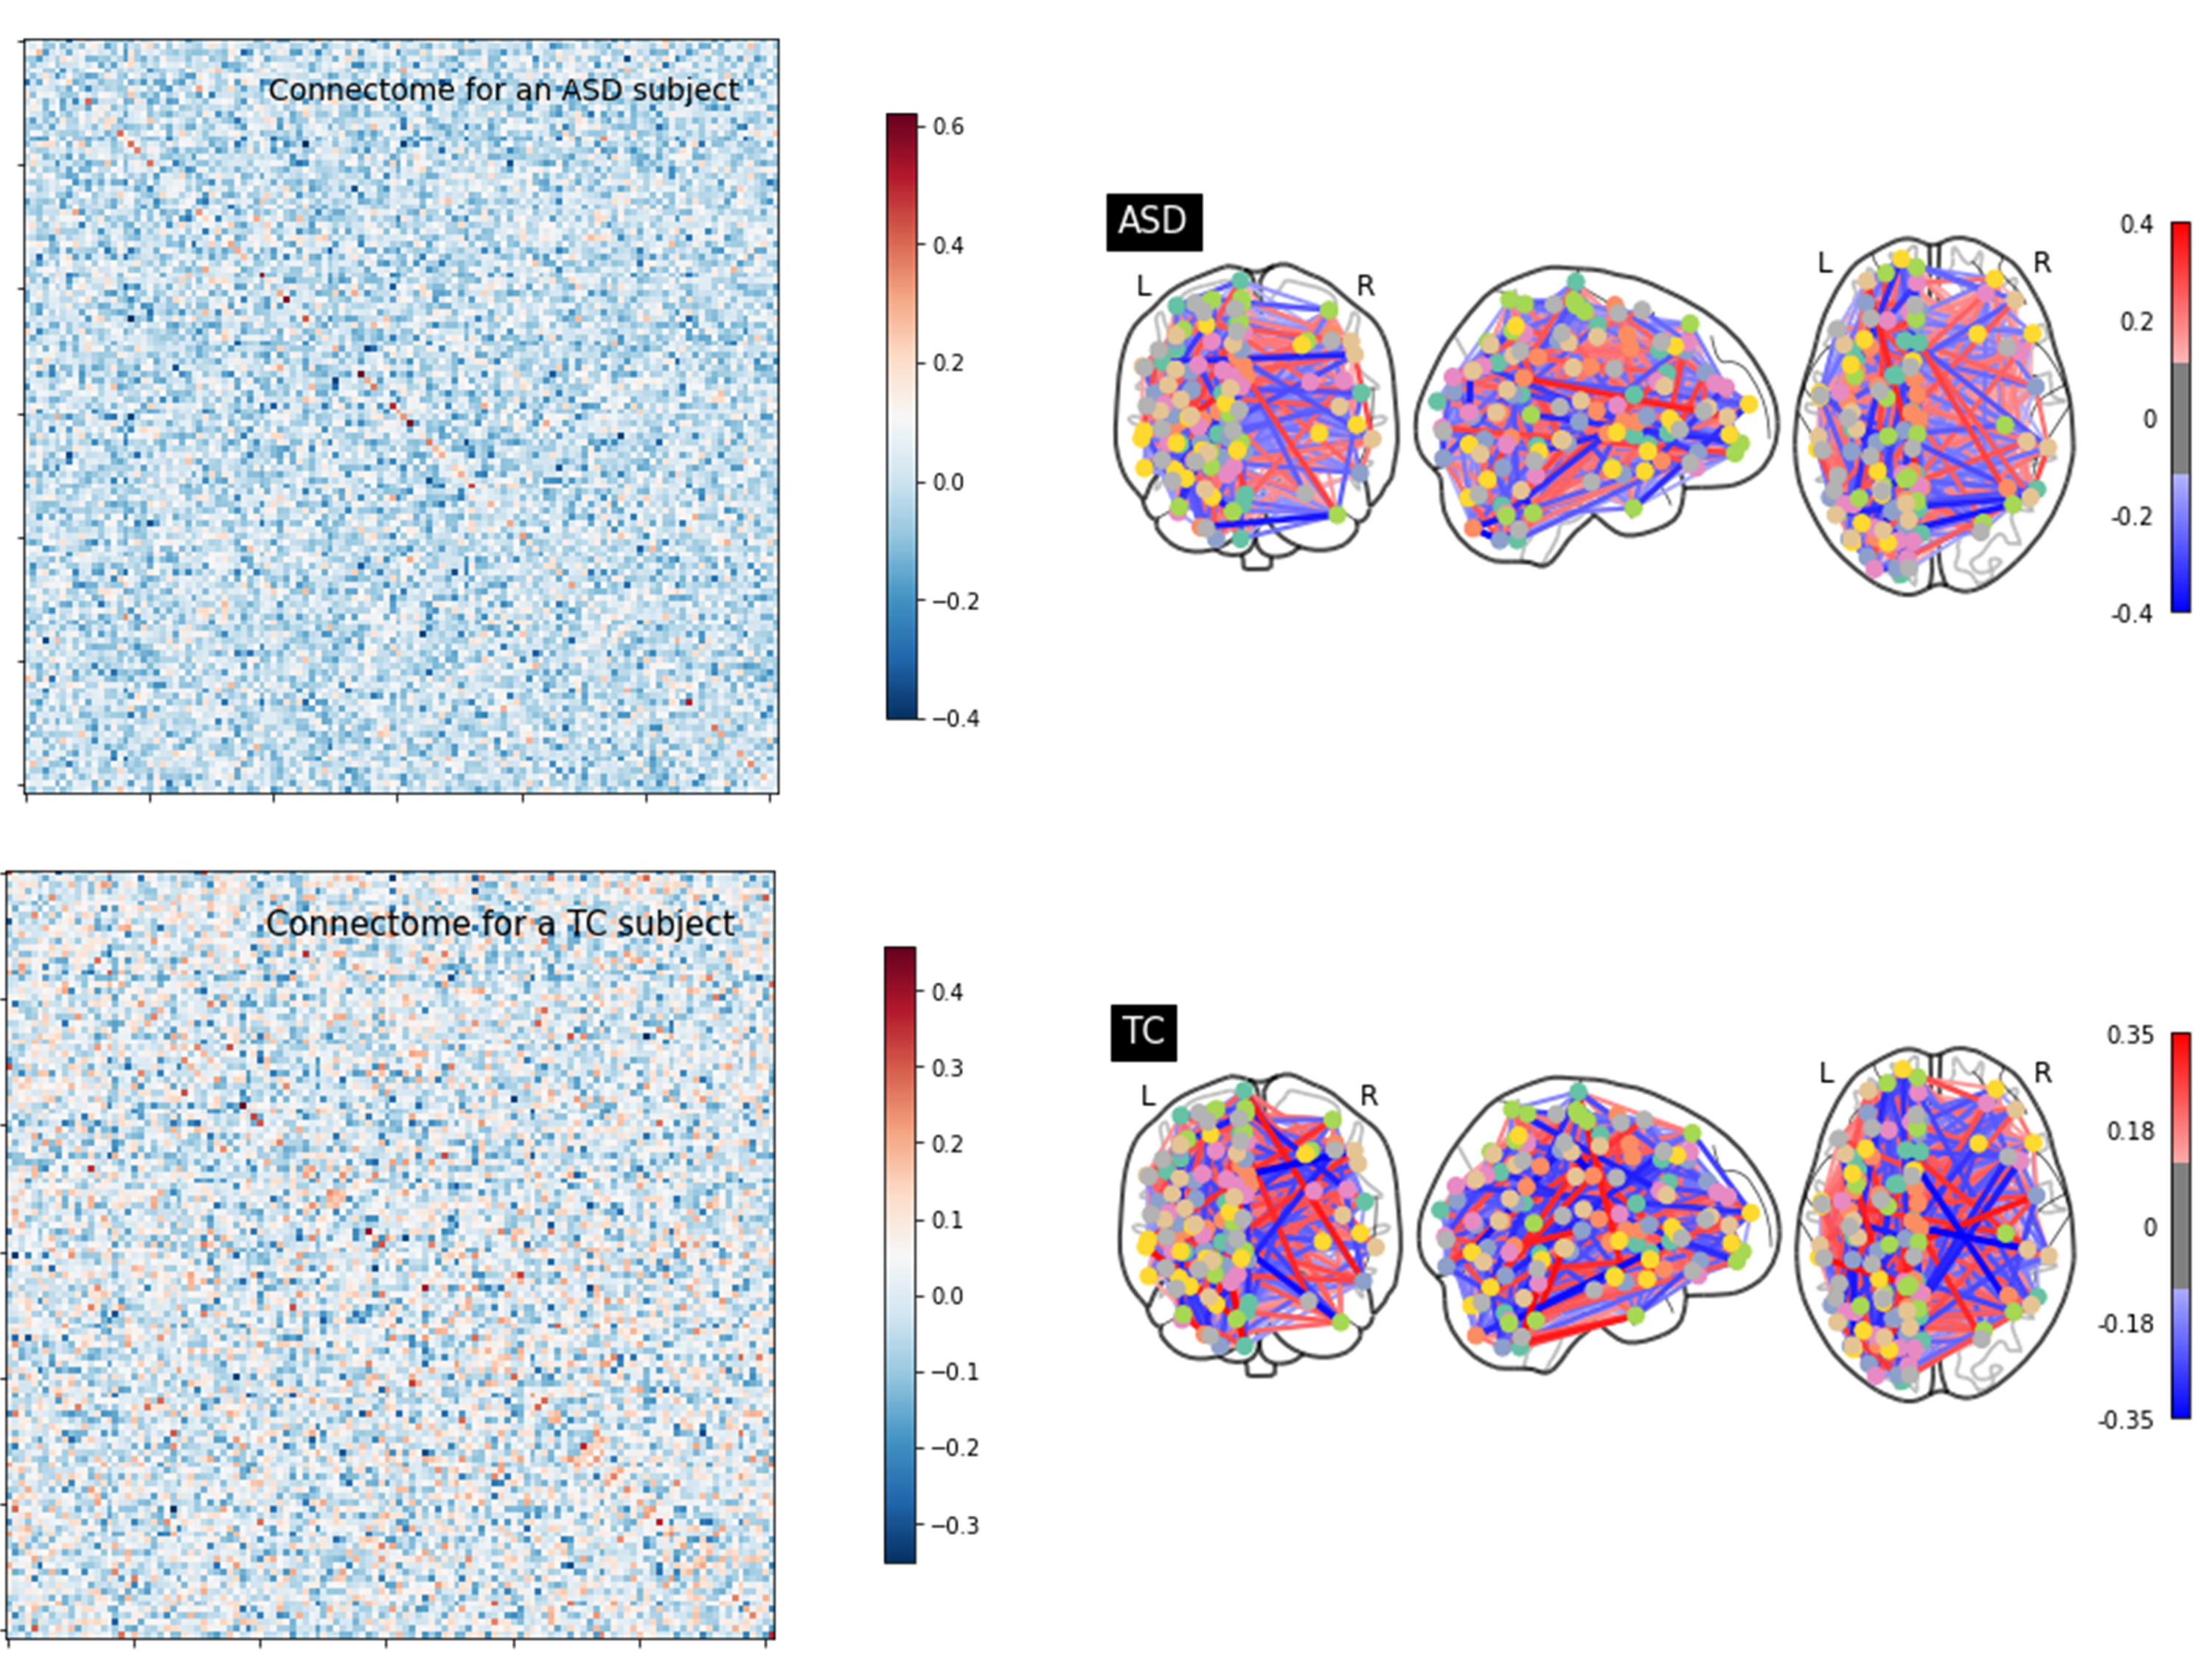
\includegraphics[width=\linewidth]{figures/Figure 3.6.png}
\caption{Difference between connectomes of random participants belonging to the ASD and control group.}
\label{fig:3.6}
\end{figure}

The connectivity matrices were plotted using the ConnectivityMeasure function belonging to the connectome class and the embedded connectome was created using the view\_connectome
function from the plotting class of Nilearn library.

\subsection{Transforming 2D Functional Connectivity Matrix to 1D Feature Vector}

The tangent connectivity matrix is symmetrical and the upper triangular value repeats the
lower one. To reduce dimensionality, we remove the upper triangular value including the
diagonal and retrieve the lower triangular value as shown in Figure \ref{fig:3.7}. Next, the lower triangular part of interest is flattened to a 1D vector of size, 
\begin{equation}
S=\frac{N(N-1))}{2}
\label{S_equation}
\end{equation}
where N = number of ROIs. Thus, using the stated atlases, we received a feature vector of size 19,900, 6670, 7381, and 34,716, respectively, for CC200, AAL, BASC, and Power atlases in the case of each subject.\\

\begin{figure}[h!]
\centering
\includegraphics[width=\linewidth]{figures/Figure 3.7.png}
\caption{Retrieval of lower triangular part from symmetrical connectivity matrix.}
\label{fig:3.7}
\end{figure}

\subsection{Classification}

Classification is the process of assigning an unknown sample to a pre-defined class or label
after training the classifier on a set of training data. Performance of machine learning
classifiers such as \Gls{KNN}, Random Forest, Naïve Bayes, etc to successfully predict functional
connectivity-based classification have been compared across rs-fMRI cohorts by Dadi et
al. \cite{dadi2019benchmarking}. To our knowledge, no comparative analysis has been conducted using deep learning
classifiers and multiple atlases to outline the impact of modelling choices on predicting over
diverse phenotypes, as of now. Hence, in this study, we perform the classification task using
a DNN (Deep Neural Network) classifier.\\

Deep neural networks, also termed as Feed-Forward Networks are supervised learning-based
classifiers in which data flow is unidirectional from input to the output layer and consists of
at least two hidden layers. The outputs are obtained by backpropagation. The
backpropagation technique performs fine-tuning of the weights of a neural network to output
the expected class minimizing prediction error. The hyperparameters involved in this
classification are described in the following subsections along with their mathematical basis.

\subsubsection{Hidden Layers and Number of Neurons}
The obtained feature vectors were provided as input to the proposed deep neural network classifier (DNN). The proposed DNN (referred as Model-2 in the later sections) consisted of two hidden layers with 32 neurons per layer, as illustrated in Figure \ref{fig:3.8}.

\begin{figure}[hbt!]
\centering
\includegraphics[scale=0.5]{figures/Figure 3.8.png}
\caption{Proposed deep neural network architecture to predict ASD.}
\label{fig:3.8}
\end{figure}

Other configurations with more than 2 hidden
layers were also attempted but experimental results decreased due to lack of training samples.

\subsubsection{Activation Function}

Activation functions help the network learn complex patterns in the data and transforms the
output of the network within a certain range which aids in making effective predictions. In
this, network, the hidden layers use relu activation and the final output layer uses the sigmoid
activation function.\\

Let, $x\textsubscript{i}$ and $b\textsubscript{i}$ be the input and bias value of layer $i$ respectively, $W\textsubscript{i}$ is the weight vector
connecting the nodes in layer $i$ to the nodes in layer $i+1$, then, layer $i+1$ is activated using
the following equation \ref{activation_equation}:

\begin{equation}
Z_{i+1}=f(W_{i}x_{i}+b_{i})
\label{activation_equation}
\end{equation}

where $Z$ denotes activation of the subscripted hidden layer and $f$ is the ReLU activation function defined in equation \ref{relu_equation}: 

\begin{equation}
f(x)=max⁡(0,x)
\label{relu_equation}
\end{equation}

In the case of sigmoid,

\begin{equation}
f(x)=\frac{1}{1+e{^{-x}}}
\label{sigmoid_equation}
\end{equation}

where $e$ = Euler’s number. It exists between 0 and 1 and predicts the probability value as an output in the case of binary classification.

\subsubsection{Optimizer}
The function of an optimizer is to change attributes like weight and learning rate to reduce
losses. Adam optimizer has been used in this regard with a relatively low learning rate of
0.0001. Adam is an adaptive learning rate optimization algorithm which can be considered a
combination of RMSProp and SGD with momentum.

\subsubsection{Loss Function}
The binary cross-entropy loss function is used in this binary classification problems (autism vs
control). This loss function is defined in equation \ref{cost_equation}:

\begin{equation}
J=-\frac{1}{m}\sum_{i=1}^{m}[y_{i}\cdot\log({p({y_{i}})})+(1
-y_{i})\cdot\log({p({1-y_{i}})})]
\label{cost_equation}
\end{equation}

Where $m$ is the total number of samples, $y$ is the label and $p$ indicates the probability of $y$
belonging to autism or control group. The objective of the network is to minimize the value
of loss function, $J$.\\

\subsubsection{Regularizer}
Since our input vector is high dimensional, we employed regularization techniques so that our
model generalizes well, reduces the chance of overfitting and performs better on unseen data
as well.

\begin{itemize}
    \item \textbf{L2 Regularizer:} Also termed as weight decay, it updates the general cost function by adding another
component or a regularized term to penalize large weights. Thus,\\
Cost Function = Binary cross-entropy loss + Regularization term

\item \textbf{Dropout:} A dropout layer randomly selects some neurons/nodes and removes them at every
iteration. Dropout layers with a dropout probability of 0.8 were used.
\end{itemize}

\subsubsection{Batch Size}
It refers to training samples utilized per iteration. A batch size of 10 has been used in this
case. The reason for such a small batch size is to obtain a regularization effect and reduce
generalization error.

\subsubsection{Callback Functions}
While training the neural network, we use the following Keras callback functions that enable
us to interact with the process of training the model by providing a view of the internal states
during training. The following callbacks were used.

\begin{itemize}
\item \textbf{Early Stopping:} The early stopping method allows us to choose a large random number of epochs
while training. When the model performance stops improving on a validation set,
training halts. This reduces the task of declaring a random number of epochs
before training and fine-tuning it again and again. In this model, early stopping
monitored validation loss with patience=5. If validation loss stopped decreasing
after 5 consecutive epochs, training stops.

\item \textbf{Model Checkpoint:} This function enables us to resume the training process in case of interruption and
also use a pre-trained model without having to train it again by saving the model weights after every epoch. We set save\_best\_only = True, i.e, we save only the
latest best weights while training the model by monitoring validation accuracy.

\end{itemize}

\section{Conclusion}
The methodology of our proposed deep learning-based procedure to identify ASD has been
discussed in detail in this chapter. For extraction of time-series data, four standard predefined
atlases were used. For functional connectivity computation, tangent space embedding was
performed. The upcoming chapter contains detailed descriptions of the experimental result
analyses on the proposed framework.